\section{Vyvážené stromy}

Pôvodná verzia \citep{kuko} obsahovala vizualizáciu viacerých vyvážených stromov.
K nim sme pridali \Bp-stromy, stromy s prstom a stromy s reverzami.

\subsection{B$\!^+\!$-strom}

\paragraph{Popis.}
\emph{\Bp-strom} je variácia B-stromu, v ktorom sú všetky kľúče uložené v listoch
a listy sú pospájané do spájaného zoznamu. Prvky vo vnútorných vrcholoch slúžia len
na navigáciu. 

\Bp-strom rádu $b$ je strom, v ktorom má každý vnútorný vrchol najviac $b$
a najmenej $\lfloor b/2 \rfloor$ synov (okrem koreňa, ktorý má najmenej dvoch synov).
Vďaka tomu je dobre vyvážený a jeho operácie sú vykonávané v logaritmickom čase.
\Bp-strom je \emph{asociatívne pole (slovník)}, čiže poskytuje tieto tri operácie:
\begin{itemize}
\item $\ins(x)$ -- pridá do stromu prvok $x$;
\item $\find(x)$ -- zistí, či sa $x$ v strome nachádza;
\item $\delete(x)$ -- odstráni $x$ zo stromu.
\end{itemize}

Operácia $\find(x)$ začne v koreni, nájde v ňom prvý kľúč väčší od hľadaného.
Nech je $i$-ty v poradí, potom hľadanie pokračuje $i$-tou vetvou.
(Ak je $x$ väčšie ako všetky kľúče, pokračujeme poslednou vetvou.)
V liste už len skontrolujeme, či sa v ňom hľadaný kľúč nachádza.

% Definujeme dve operácie: {\sc Copy-Up} a {\sc Push-Up}, ktoré používa operácia $\ins$.
% Ak má vrchol viac prvkov, ako je maximálny limit, treba ho zmenšiť. Rozdelí sa na dve časti.
% Ak vrchol nie je listom, použije sa {\sc Push-Up}, najmenší kľúč pravej časti sa vyberie
% a stane sa otcom vytvorených dvoch častí. Pokiaľ to list je, kľúč v ňom musí zostať,
% preto sa iba skopíruje. Táto operácia sa nazýva {\sc Copy-Up}.

Operácia $\ins(x)$ najprv pomocou operácie $\find$ zistí, či štruktúra daný kľúč už obsahuje.
Ak nie, je zrejmé, že $x$ patrí práve na miesto, kde $\find$ skončil.
Môže sa stať, že vrchol po vložení "pretečie" -- bude obsahovať $b+1$ prvkov. V takom prípade
ak má vrchol brata s menej ako $b$ prvkami, môžeme jeden kľúč presunúť k nemu.
Ak sú susedné vrcholy plné, vrchol rozdelíme na dva, pričom stredný kľúč skopírujeme
k otcovi. (Ten sa môže tiež preplniť -- môže vzniknúť celá kaskáda rozdelení, ktorá skončí
v najhoršom prípade v koreni.)
% Nový vrchol s jedným kľúčom, ktorý vznikol, vložíme do
% otcovského vrcholu. Ak otcovský vrchol presiahol najväčšiu možnú veľkosť, znova sa aplikuje
% popísaný algoritmus s jedným rozdielom -- namiesto {\sc Copy-Up} sa použije {\sc Push-Up}.

Podobne v operácií $\delete$ môže vrchol "podtiecť". Ak má suseda s aspoň $\lfloor b/2 \rfloor+1$
kľúčmi, môže si jeden požičať od neho. V opačnom prípade môžeme vrchol s jeho susedom zlúčiť.
% najprv pomocou $\find$ nájde kľúč, potom ho z vrcholu odstráni. Tento vrchol
% môže mať po odstránení menší počet kľúčov ako minimálny limit. Vtedy, ak sa dá, sa prenesie
% jeden kľúč zo súrodenca. Ak sa nedá, vrchol sa s ním zlúči. Zároveň sa k nim pridá aj kľúč
% z otcovského vrcholu, ktorý ich rozdeľoval. Pokiaľ to spôsobilo, že otcovský vrchol má menej
% kľúčov, ako je povolené, znova sa aplikuje predošlý algoritmus. Keďže na koreň sa nevzťahuje
% minimálny limit, po skončení bude strom zaručene v konzistentnom tvare.

\paragraph{Časová zložitosť a použitie.}
\Bp-stromy sú vhodnou dátovou štruktúrou pre dáta uložené na disku: keďže dĺžka prístupu na
disk je v porovnaní s výpočtami v hlavnej pamäti veľmi veľká, snažíme sa ich počet minimalizovať.
Hoci časová zložitosť všetkých operácií je $O(b\log_b n)$, potrebujeme iba $O(\log_b n)$ prístupov
na disk. Ak zvolíme vhodný rád, vieme jednotlivé vrcholy dobre napasovať na stránky a tým regulovať
ako počet prístupov k pamäti, tak jej zaplnenie.

Hlavné využitie \Bp-stromov je v databázových systémoch. Stromy vieme rozšíriť tak, aby podporovali
rôzne agregačné funkcie, ako napríklad súčet, minimum, či priemer daného intervalu pomocou $O(\log_b n)$
prístupov na disk. Vypísať všetky prvky z daného intervalu dokážeme pomocou $O(\log_b n + t/b)$ prístupov na disk.
% \Bp-strom podporuje efektívne vyhľadanie prvkov poľa, ktoré patria do daného intervalu.
% Algoritmus nájde jeden krajný bod a vďaka spájanému zoznamu, vytvorenému z listov, ostatné prvky
% postupne prečíta. Zložitosť je $O(\log_b(n) + t/b)$, kde $t$ je počet výsledných kľúčov z hľadaného intervalu.

Ďalšia výhoda \Bp-stromov oproti B-stromom sa prejaví, ak máme utriedený zoznam dát a chceme z neho vytvoriť \Bp-strom:
\Bp-strom môžeme vystavať odspodu. Takýto postup vyžaduje $O((n/b)\cdot\log_b n)$ prístupov na disk,
čo je $b$-krát rýchlejšie ako spraviť $n$ volaní $\ins$.

\begin{figure*}
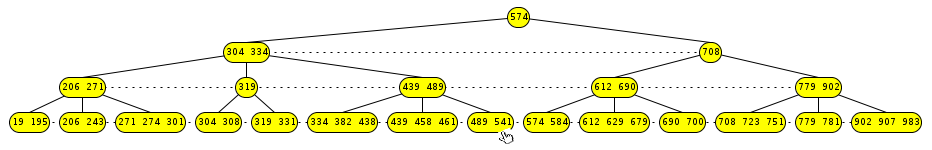
\includegraphics[width=2\columnwidth]{obrazky/finger.png}
\caption{\emph{Strom s prstom.} Jednotlivé kľúče sú uložené v listoch, vnútorné vrcholy
slúžia na vyhľadávanie. Vďaka smerníkom spájajúcim vrcholy na jednej úrovni vieme nájsť
ľubovoľný prvok vo vzdialenosti $d$ od prstu v čase $O(\log d)$.}
\label{img:finger}
\end{figure*}

\subsection{Strom s prstom}
Tradičné vyvážené vyhľadávacie stromy podporujú vyhľadávanie v čase $O(\log n)$.
Prst je smerník na konkrétny vrchol, ktorý umožňuje efektívnejší prístup k vrcholom
v jeho blízkom okolí. Hovoríme, že vyhľadávací strom podporuje vyhľadávanie s prstom
(tzv.\ \emph{finger search tree}), ak kľúč vo vzdialenosti $d$ dokážeme nájsť v čase $O(\log d)$.
Špeciálne predchodcu a následníka vieme nájsť v konštantnom čase.

Existuje viacero riešení, ktoré podporujú vyhľadávanie s prstom, v našom programe
sme implementovali upravený 2-3-4$^+$ strom \citep{finger}.

\paragraph{Popis.}
2-3-4$^+$ strom je \Bp-strom rádu 4, t.j.\ kľúče sú uložené v listoch a vnútorné vrcholy
majú stupeň 2, 3 alebo 4. Pre podporu vyhľadávania s prstom spojíme všetky vrcholy
na rovnakej úrovni (v rovnakej vzdialenosti od koreňa) do obojsmerného spájaného zoznamu.
Ak sú nejaké dva vrcholy spojené takouto hranou, budeme hovoriť, že sú susedia (pozri
obr.~\ref{img:finger}).

% Prst, ako už bolo spomenuté, ukazuje na nejaký vrchol. Môže sa pohybovať po všetkých hranách
% a pomocou neho sa vykonávajú všetky operácie. Keďže sú všetky kľúče uložené v listoch, prst
% na tejto vrstve začína, aj končí.

Operácia $\find$ začína vo vrchole, kam ukazuje prst. Vyhľadávanie pozostáva z dvoch
fáz: V prvej fáze postupujeme nahor, až kým hľadaný kľúč nepatrí do nášho alebo susedovho podstromu.
(V prípade potreby použijeme úrovňovú hranu, ktorou sa dostaneme do susedného vrcholu.)
V druhej fáze potom zostupujeme nadol ako pri štandardnom vyhľadávaní.
Pri $\ins$ a $\delete$ najskôr pomocou prstu nájdeme vhodné miesto a následne kľúč pridáme/vymažeme,
rovnako ako v \Bp-strome. 

Takto implementované vyhľadávanie trvá $O(\log d)$, vkladanie a vymazávanie (po tom ako sme vrchol
našli) má konštantnú amortizovanú zložitosť.


% Skontroluje, či by kľúč mal patriť do daného
% vrcholu. Ak nie, pozrie sa, či nepatrí do niektorého zo susedov. Ak áno, prst sa tam presunie
% a vyhľadávanie sa skončilo. Inak smerník prejde o úroveň vyššie, na otcovský vrchol. Ak hľadaný
% kľúč patrí do jeho podstromu (t.j.\ je väčší ako jeho najmenší kľúč a menší ako ten najväčší),
% zíde po hranách do listu, kde by sa daný kľúč mal nachádzať. Keď do podstromu nepatrí, skontroluje,
% či nepatrí do podstromu susedov. Ak áno, prejde po vrstevnej hrane na suseda a následne zíde až
% do listu, kde by mal kľúč byť. Pokiaľ prst nenarazil na správny podstrom, znova sa presunie smerom
% nahor po otcovskej hrane. Hľadanie pokračuje analogicky.
%Je zrejmé, že ak prst ukazuje na koreň, kľúč bude patriť do jeho podstromu.

% Otázka patričnosti do podstromu sa dá pre krajné prípady optimalizovať. Ak totiž vrchol, na ktorý
% ukazujeme, nemá napríklad pravého suseda, je zrejmé, že vačší kľúč ako je najvačší v tomto vrchole
% v strome nie je. Preto ľubovoľný kľúč do podstromu tohto vrcholu patrí práve vtedy, keď je väčší
% ako jeho najmenší prvok. Analogicky to platí, ak chýba ľavý sused.
% 
% Operácia $\ins$ najprv pomocou operácie $\find$ nájde miesto, kam by mal vkladaný kľúč patriť. 
% Ak taký kľúč už v strome je, ďalší sa nevloží. V prípade, že sme vložili nový kľúč, môže sa stať, 
% že vrchol "pretečie", tzn.\ má viac ako 3 prvky%
% (pozri obr.~\ref{img:finger-insert}). Situácia sa vyrieši rovnako ako v \Bp-strome. 

% Operácia $\ins$ najprv pomocou operácie $\find$ zistí, či štruktúra daný kľúč obsahuje. Ak nie, 
% je zrejmé, že patrí práve do vrcholu, kde $\find$ skončil. V prípade, že sme vložili nový kľúč, 
% môže sa stať, že vrchol "pretečie", tzn.\ má viac ako 3 prvky %
% (pozri obr.~\ref{img:finger-insert}). Ak vrchol pretiekol, použije sa {\sc Copy-Up}
% a rozdelí sa na dve časti. Stredný jednoprvkový vrchol sa vloží do otca. Ak pretiekol, použijeme 
% rovnaký postup, akurát s {\sc Push-Up}. Pokračujeme analogicky, pokým štruktúra nebude znova 
% v konzistentom stave.

% \begin{figure}
% 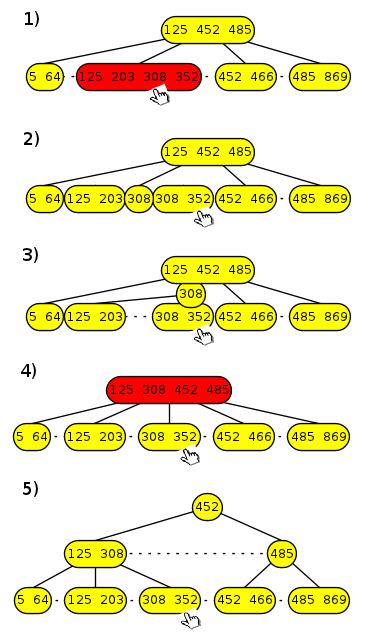
\includegraphics[width=\columnwidth]{obrazky/finger-insert.png}
% \caption{\emph{Pretečenie vrcholu.} Do stromu sme vložili prvok $308$ a 1) listový vrchol pretiekol. 
% 2) vrchol sa delí a kľúč sa kopíruje, aby originál zostal v liste 3) nový otec sa vkladá do vyššej vrstvy 
% 4) aj tento vrchol preteká, delí sa a vzniká nový koreň 5) finálny tvar.}
% \label{img:finger-insert}
% \end{figure}
% 
% Operácia $\delete$ najprv pomocou operácie $\find$ nájde miesto, kam by mal hľadaný kľúč patriť. 
% Ak tam nie je, vymazávanie sa končí. Inak sa vymaže. Môže sa stať, že vrchol "podtečie", tzn.\ 
% nemá kľúč. Tento problém sa rieši rovnako ako v \Bp-strome. 
% Samozrejme je treba ošetriť konzistentnosť vo vyšších vrstvách, aby sa tam nenachádzali kópie 
% kľúčov, ktoré už boli zo štruktúry vymazané (pozri obr.~\ref{img:finger-delete}).  
% 
% \begin{figure}
% 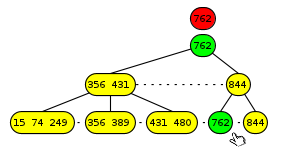
\includegraphics[width=\columnwidth]{obrazky/finger-delete.png}
% \caption{\emph{Vymazávanie kľúča $762$.} Odstrániť sa musí aj kópia vo vyšších vrstvách.}
% \label{img:finger-delete}
% \end{figure}
% 
% \paragraph{Časová zložitosť.}
% Keďže každý vrchol má aspoň dvoch synov, 2-3-4 strom má hĺbku $O(\log n)$, kde $n$ je počet kľúčov, 
% a teda podporuje vykonávanie operácií v čase $O(\log n)$. Ak sa však použije prst, časová zložitosť 
% vychádza na $O(\log d)$, kde $d$ je vzdialenosť pozície prsta a vrcholu, kam patrí cieľový kľúč, 
% amortizovane dokonca na $O(1)$ \citep{sahni}.

% \paragraph{Použitie.}
% Prst ako smerník na prvok štruktúry, ktorý umožňuje efektívnejší prístup k okolitým kľúčom, prvýkrát
% spomenuli Guibas et al. Vo svojej publikácii prezentujú B-strom podporujúci vyhľadávanie v $O(\log n)$
% a update-y dokonca v $O(1)$ čase, predpokladajúc, že je udržiavaných len $O(1)$ pohyblivých prstov \citet{sahni}.
% Pohyb prsta o $d$ pozícií trvalo $O(\log n)$ času. Na základe tejto práce navrhli Huddleston a Mehlhorn
% svoj vrstvovo spájaný 2-3-4 strom, ktorý bol neskôr upravený vďaka Belloch et al. na priestorovo efektívnejšiu
% alternatívu. Toto riešenie využíva jeden prst, s ktorým štruktúra ponúka rovnakú operačnú zložitosť ako 2-3-4 stromy.
% %Model bol dokonca zovšeobecnený na ($a$,$b$)-stromy, kde $b\geq 2a$.
% %Je zaujímavé, že pre 2-3 strom bola nájdená postupnosť vkladaní a vymazávaní, ktorá vyžaduje $\Omega(n\log n)$ krokov \citet{sahni}.

% \paragraph{Vizualizácia.}
% Strom s prstom je vizualizovaný pomocou \Bp-stromu s rádom 4, keďže jeho podmienky pre počet potomkov vyhovujú
% danej štruktúre.
% Prst je samostaný pohyblivý článok, ktorý si pamätá iba vrchol, na ktorý ukazuje. Po stromovitej
% štruktúre sa vie hýbať vďaka informáciám získaným z daného vrcholu.

\subsection{Strom s reverzami}
\emph{Strom s reverzami} je dátová štruktúra na uchovávanie permutácií. 
Majme permutáciu $\pi$ na množine $\{1,2,\ldots,n\}$; dátová štruktúra
poskytuje operácie 
\begin{itemize}
%\item $\ins(k)$ -- pridá do stromu $k$;
\item $\reverse(i,j)$ -- preklopí poradie prvkov v intervale od $i$ po $j$,
\item $\find(k)$ -- zistí, ktorý prvok je na $k$-tom mieste permutácie $\pi$.
\end{itemize}

\paragraph{Popis.}
Permutáciu reprezentujeme ako strom, v ktorom je \emph{inorder} poradie prvkov totožné 
s poradím prvkov v permutácií. Strom s reverzami môžeme implementovať pomocou ľubovoľného 
vyváženého stromu, ktorý podporuje rozdelenie a zreťazenie dvoch stromov v logaritmickom čase. 
My sme zvolili \emph{splay strom} pre jeho jednoduchosť. 

% Splay strom je štruktúrou binárny strom,
% líši sa od neho iba operáciami. Keď pracuje s ľubovoľným prvkom, na konci operácie bude vo vrchole
% buď daný kľúč alebo najbližší z jeho okoli. Na rozdiel od splay stromu, strom s reverzami nepracuje
% s kľúčmi, ale s poradím prvkov. Preto je nutné, aby mal

Niektoré vrcholy môžu byť označené vlajkou, ktorá signalizuje, že celý podstrom je reverznutý a 
prvky sú v skutočnosti v opačnom poradí (pozri obr.~\ref{img:rev1}).

Operáciu $\reverse$ implementujeme lenivo: 
strom najskôr rozdelíme na tri časti: $T_1,T_2,T_3$, pričom $T_2$ obsahuje interval od $i$-teho 
po $j$-ty prvok, $T_1$ obsahuje začiatok a $T_3$ koniec permutácie (obr.~\ref{img:rev2}). 
Koreň $T_2$ jednoducho označíme vlajkou. Ak už koreň vlajku obsahuje, odstránime ju. 
Následne stromy $T_1,T_2,T_3$ opäť spojíme.

Aby sme vedeli efektívne vyhľadať $k$-ty prvok, budeme si pre každý vrchol udržiavať veľkosť jeho
podstromu. V operácií $\mathop{\mathit{find}}(k)$ sa vieme podľa toho rozhodnúť, či sa $k$-ty prvok nachádza v ľavom podstrome,
resp.~koľký prvok je v pravom podstrome. (Po nájdení sa prvok presunie do koreňa pomocou operácie splay.)

\begin{figure}
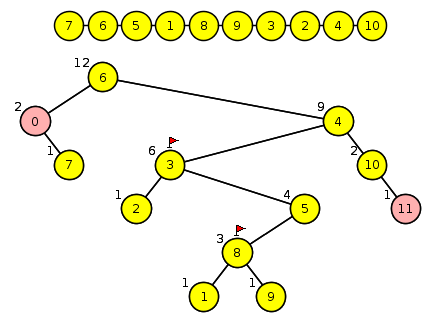
\includegraphics[width=\columnwidth]{obrazky/rev1.png}
\caption{\emph{Strom s reverzami.} Hore permutácia $\pi$, dolu jej reprezentácia pomocou splay stromu.
Vlajky vo vrcholoch 3 a 8 signalizujú, že v inorder poradí vrcholov $7,6,\underline{2,3,\underline{1,8,9},5},4,10$
treba podčiarknuté úseky (zodpovedajúce podstromom 3 a 8) prevrátiť.
Číslo vľavo hore od vrcholu je počet vrcholov v danom podstrome.}
\label{img:rev1}
\end{figure}

Pri takomto riešení musíme ešte upraviť vyhľadávanie a rotácie, aby brali do úvahy vlajky vo vrcholoch.
Najelegantnejšie riešenie je odstrániť vlajku vždy, keď na ňu narazíme:
Danému vrcholu odstránime vlajku, vymeníme mu synov a každému synovi vlajkový bit znegujeme.

Všetky operácie vieme implementovať v rovnakom čase ako operácie v splay tree, teda amortizovaná 
časová zložitosť oboch operácií je $O(\log n)$.

\paragraph{Použitie.}
Stromy s reverzami (pôvodne založené na AVL stromoch) navrhli \citet{chrobak}
na efektívnu implementáciu 2-opt heuristiky na riešenie problému obchodného cestujúceho.
Pri 2-opt heuristike sa snažíme preklápať rôzne úseky cesty, kým nenájdeme lokálne minimum.

V bioinformatike sa tieto stromy používajú na triedenie orientovaných permutácií
pomocou reverzov \citep{reversals,reversals2}.

Za povšimnutie stojí fakt, že táto dátová štruktúra podporuje výmenu ľubovoľných dvoch blokov
v logaritmickom čase, keďže túto operáciu vieme odsimulovať pomocou štyroch reverzov.

\paragraph{Vizualizácia.}
Pre lepšiu predstavu, bolo pridané pole, v ktorom užívateľ vidí skutočné poradie prvkov, ktoré
zo stromu nie je až tak zjavné (obr.~\ref{img:rev1}, \ref{img:rev2}). Pole simuluje operácie spolu so stromom,
tie sa však vykonávajú v lineárnom čase.

Do stromu sme pridali ako zarážky prvky 0 a $n+1$. Tieto prvky do reverzovateľného
intervalu nepatria, majú však zmysel v prípade, ak sa reverzuje interval, ktorý zahŕňa
aspoň jeden okraj: V tom prípade v operácii $\reverse$ nezostane $T_1$ ani $T_3$ prázdny. 
%Aby nevznikli problémy s operáciami, za krajné kľúče boli zvolené hodnoty $0$ a číslo o jedna väčšie od aktuálneho maxima.

\begin{figure}
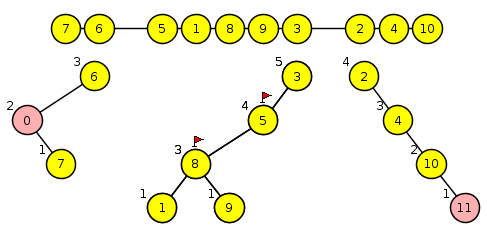
\includegraphics[width=\columnwidth]{obrazky/rev2.png}
\caption{Pri operácii \emph{reverse} sa strom rozdelí na tri časti. 
Vľavo sú prvky pred intervalom, vpravo prvky za ním. 
Na prevrátenie úseku $5,1,8,9,3$ stačí pridať vlajku vrcholu 3 (koreň stredného stromu)
a stromy opäť spojiť.}
\label{img:rev2}
\end{figure}

